
\let\negmedspace\undefined
\let\negthickspace\undefined
\documentclass[journal,12pt,twocolumn]{IEEEtran}

%
\usepackage{setspace}
\usepackage{gensymb}
%\doublespacing
\singlespacing

%\usepackage{graphicx}
%\usepackage{amssymb}
%\usepackage{relsize}
\usepackage[cmex10]{amsmath}
%\usepackage{amsthm}
%\interdisplaylinepenalty=2500
%\savesymbol{iint}
%\usepackage{txfonts}
%\restoresymbol{TXF}{iint}
%\usepackage{wasysym}
\usepackage{amsthm}
%\usepackage{iithtlc}
\usepackage{mathrsfs}
\usepackage{txfonts}
\usepackage{stfloats}
\usepackage{steinmetz}
\usepackage{bm}
\usepackage{cite}
\usepackage{cases}
\usepackage{subfig}
%\usepackage{xtab}
\usepackage{longtable}
\usepackage{multirow}
%\usepackage{algorithm}
%\usepackage{algpseudocode}
\usepackage{enumitem}
\usepackage{mathtools}
\usepackage{tikz}
\usepackage{circuitikz}
\usepackage{verbatim}
\usepackage{tfrupee}
\usepackage[breaklinks=true]{hyperref}
%\usepackage{stmaryrd}
\usepackage{tkz-euclide} % loads  TikZ and tkz-base
%\usetkzobj{all}
\usepackage{listings}
    \usepackage{color}                                            %%
    \usepackage{array}                                            %%
    \usepackage{longtable}                                        %%
    \usepackage{calc}                                             %%
    \usepackage{multirow}                                         %%
    \usepackage{hhline}                                           %%
    \usepackage{ifthen}                                           %%
  %optionally (for landscape tables embedded in another document): %%
    \usepackage{lscape}     
\usepackage{multicol}
\usepackage{chngcntr}
%\usepackage{enumerate}

%\usepackage{wasysym}
%\newcounter{MYtempeqncnt}
\DeclareMathOperator*{\Res}{Res}
%\renewcommand{\baselinestretch}{2}
\renewcommand\thesection{\arabic{section}}
\renewcommand\thesubsection{\thesection.\arabic{subsection}}
\renewcommand\thesubsubsection{\thesubsection.\arabic{subsubsection}}

\renewcommand\thesectiondis{\arabic{section}}
\renewcommand\thesubsectiondis{\thesectiondis.\arabic{subsection}}
\renewcommand\thesubsubsectiondis{\thesubsectiondis.\arabic{subsubsection}}

% correct bad hyphenation here
\hyphenation{op-tical net-works semi-conduc-tor}
\def\inputGnumericTable{}                                 %%

\lstset{
%language=C,
frame=single, 
breaklines=true,
columns=fullflexible
}
%\lstset{
%language=tex,
%frame=single, 
%breaklines=true
%}

\begin{document}
%


\newtheorem{theorem}{Theorem}[section]
\newtheorem{problem}{Problem}
\newtheorem{proposition}{Proposition}[section]
\newtheorem{lemma}{Lemma}[section]
\newtheorem{corollary}[theorem]{Corollary}
\newtheorem{example}{Example}[section]
\newtheorem{definition}[problem]{Definition}
%\newtheorem{thm}{Theorem}[section] 
%\newtheorem{defn}[thm]{Definition}
%\newtheorem{algorithm}{Algorithm}[section]
%\newtheorem{cor}{Corollary}
\newcommand{\BEQA}{\begin{eqnarray}}
\newcommand{\EEQA}{\end{eqnarray}}
\newcommand{\define}{\stackrel{\triangle}{=}}

\bibliographystyle{IEEEtran}
%\bibliographystyle{ieeetr}


\providecommand{\mbf}{\mathbf}
\providecommand{\pr}[1]{\ensuremath{\Pr\left(#1\right)}}
\providecommand{\qfunc}[1]{\ensuremath{Q\left(#1\right)}}
\providecommand{\sbrak}[1]{\ensuremath{{}\left[#1\right]}}
\providecommand{\lsbrak}[1]{\ensuremath{{}\left[#1\right.}}
\providecommand{\rsbrak}[1]{\ensuremath{{}\left.#1\right]}}
\providecommand{\brak}[1]{\ensuremath{\left(#1\right)}}
\providecommand{\lbrak}[1]{\ensuremath{\left(#1\right.}}
\providecommand{\rbrak}[1]{\ensuremath{\left.#1\right)}}
\providecommand{\cbrak}[1]{\ensuremath{\left\{#1\right\}}}
\providecommand{\lcbrak}[1]{\ensuremath{\left\{#1\right.}}
\providecommand{\rcbrak}[1]{\ensuremath{\left.#1\right\}}}
\theoremstyle{remark}
\newtheorem{rem}{Remark}
\newcommand{\sgn}{\mathop{\mathrm{sgn}}}
\providecommand{\abs}[1]{\left\vert#1\right\vert}
\providecommand{\res}[1]{\Res\displaylimits_{#1}} 
\providecommand{\norm}[1]{\left\lVert#1\right\rVert}
%\providecommand{\norm}[1]{\lVert#1\rVert}
\providecommand{\mtx}[1]{\mathbf{#1}}
\providecommand{\mean}[1]{E\left[ #1 \right]}
\providecommand{\fourier}{\overset{\mathcal{F}}{ \rightleftharpoons}}
%\providecommand{\hilbert}{\overset{\mathcal{H}}{ \rightleftharpoons}}
\providecommand{\system}{\overset{\mathcal{H}}{ \longleftrightarrow}}
	%\newcommand{\solution}[2]{\textbf{Solution:}{#1}}
\newcommand{\solution}{\noindent \textbf{Solution: }}
\newcommand{\cosec}{\,\text{cosec}\,}
\providecommand{\dec}[2]{\ensuremath{\overset{#1}{\underset{#2}{\gtrless}}}}
\newcommand{\myvec}[1]{\ensuremath{\begin{pmatrix}#1\end{pmatrix}}}
\newcommand{\mydet}[1]{\ensuremath{\begin{vmatrix}#1\end{vmatrix}}}
%\numberwithin{equation}{section}
\numberwithin{equation}{subsection}
%\numberwithin{problem}{section}
%\numberwithin{definition}{section}
\makeatletter
\@addtoreset{figure}{problem}
\makeatother

\let\StandardTheFigure\thefigure
\let\vec\mathbf
%\renewcommand{\thefigure}{\theproblem.\arabic{figure}}
\renewcommand{\thefigure}{\theproblem}
%\setlist[enumerate,1]{before=\renewcommand\theequation{\theenumi.\arabic{equation}}
%\counterwithin{equation}{enumi}


%\renewcommand{\theequation}{\arabic{subsection}.\arabic{equation}}

\def\putbox#1#2#3{\makebox[0in][l]{\makebox[#1][l]{}\raisebox{\baselineskip}[0in][0in]{\raisebox{#2}[0in][0in]{#3}}}}
     \def\rightbox#1{\makebox[0in][r]{#1}}
     \def\centbox#1{\makebox[0in]{#1}}
     \def\topbox#1{\raisebox{-\baselineskip}[0in][0in]{#1}}
     \def\midbox#1{\raisebox{-0.5\baselineskip}[0in][0in]{#1}}

\vspace{3cm}

\title{
%	\logo{
Quadratic Forms
%	}
}
\author{ G V V Sharma$^{*}$% <-this % stops a space
	\thanks{*The author is with the Department
		of Electrical Engineering, Indian Institute of Technology, Hyderabad
		502285 India e-mail:  gadepall@iith.ac.in. All content in this manual is released under GNU GPL.  Free and open source.}
	
}	
%\title{
%	\logo{Matrix Analysis through Octave}{\begin{center}\includegraphics[scale=.24]{tlc}\end{center}}{}{HAMDSP}
%}


% paper title
% can use linebreaks \\ within to get better formatting as desired
%\title{Matrix Analysis through Octave}
%
%
% author names and IEEE memberships
% note positions of commas and nonbreaking spaces ( ~ ) LaTeX will not break
% a structure at a ~ so this keeps an author's name from being broken across
% two lines.
% use \thanks{} to gain access to the first footnote area
% a separate \thanks must be used for each paragraph as LaTeX2e's \thanks
% was not built to handle multiple paragraphs
%

%\author{<-this % stops a space
%\thanks{}}
%}
% note the % following the last \IEEEmembership and also \thanks - 
% these prevent an unwanted space from occurring between the last author name
% and the end of the author line. i.e., if you had this:
% 
% \author{....lastname \thanks{...} \thanks{...} }
%                     ^------------^------------^----Do not want these spaces!
%
% a space would be appended to the last name and could cause every name on that
% line to be shifted left slightly. This is one of those "LaTeX things". For
% instance, "\textbf{A} \textbf{B}" will typeset as "A B" not "AB". To get
% "AB" then you have to do: "\textbf{A}\textbf{B}"
% \thanks is no different in this regard, so shield the last } of each \thanks
% that ends a line with a % and do not let a space in before the next \thanks.
% Spaces after \IEEEmembership other than the last one are OK (and needed) as
% you are supposed to have spaces between the names. For what it is worth,
% this is a minor point as most people would not even notice if the said evil
% space somehow managed to creep in.



% The paper headers
%\markboth{Journal of \LaTeX\ Class Files,~Vol.~6, No.~1, January~2007}%
%{Shell \MakeLowercase{\textit{et al.}}: Bare Demo of IEEEtran.cls for Journals}
% The only time the second header will appear is for the odd numbered pages
% after the title page when using the twoside option.
% 
% *** Note that you probably will NOT want to include the author's ***
% *** name in the headers of peer review papers.                   ***
% You can use \ifCLASSOPTIONpeerreview for conditional compilation here if
% you desire.




% If you want to put a publisher's ID mark on the page you can do it like
% this:
%\IEEEpubid{0000--0000/00\$00.00~\copyright~2007 IEEE}
% Remember, if you use this you must call \IEEEpubidadjcol in the second
% column for its text to clear the IEEEpubid mark.



% make the title area
\maketitle

\newpage

\tableofcontents

\bigskip

\renewcommand{\thefigure}{\theenumi}
\renewcommand{\thetable}{\theenumi}
%\renewcommand{\theequation}{\theenumi}

%\begin{abstract}
%%\boldmath
%In this letter, an algorithm for evaluating the exact analytical bit error rate  (BER)  for the piecewise linear (PL) combiner for  multiple relays is presented. Previous results were available only for upto three relays. The algorithm is unique in the sense that  the actual mathematical expressions, that are prohibitively large, need not be explicitly obtained. The diversity gain due to multiple relays is shown through plots of the analytical BER, well supported by simulations. 
%
%\end{abstract}
% IEEEtran.cls defaults to using nonbold math in the Abstract.
% This preserves the distinction between vectors and scalars. However,
% if the journal you are submitting to favors bold math in the abstract,
% then you can use LaTeX's standard command \boldmath at the very start
% of the abstract to achieve this. Many IEEE journals frown on math
% in the abstract anyway.

% Note that keywords are not normally used for peerreview papers.
%\begin{IEEEkeywords}
%Cooperative diversity, decode and forward, piecewise linear
%\end{IEEEkeywords}



% For peer review papers, you can put extra information on the cover
% page as needed:
% \ifCLASSOPTIONpeerreview
% \begin{center} \bfseries EDICS Category: 3-BBND \end{center}
% \fi
%
% For peerreview papers, this IEEEtran command inserts a page break and
% creates the second title. It will be ignored for other modes.
%\IEEEpeerreviewmaketitle

\begin{abstract}
This book provides a computational approach to school geometry based on the NCERT textbooks from Class 6-12.  Links to sample Python codes are available in the text.  
\end{abstract}
Download python codes using 
\begin{lstlisting}
svn co https://github.com/gadepall/school/trunk/ncert/computation/codes
\end{lstlisting}

\section{Examples}
\renewcommand{\theequation}{\theenumi}
\begin{enumerate}[label=\thesection.\arabic*.,ref=\thesection.\theenumi]
\numberwithin{equation}{enumi}

\input{./circle/circle_geo_exam.tex} 
\input{./conics/conics_exam.tex} 
\input{./conics/conics.tex} 

\end{enumerate}

\section{Exercises}
\renewcommand{\theequation}{\theenumi}
\begin{enumerate}[label=\thesection.\arabic*.,ref=\thesection.\theenumi]
\numberwithin{equation}{enumi}
%\renewcommand{\theequation}{\theenumi}
%\begin{enumerate}[label=\arabic*.,ref=\thesubsection.\theenumi]
%\numberwithin{equation}{enumi}

\item Find the equation of the circle passing through \myvec{0\\0} and making intercepts a and b on the coordinate axes.
\\
\solution
Let 
\begin{align}
 \vec{A}=\myvec{a\\0} ,
 \vec{B}=\myvec{b\\0},
 \vec{C}=\myvec{0\\0}
\end{align}
Since the circle passes through $\myvec{0\\0}$, the equation of given circle is,
\begin{align}
    \vec{x^\top}\vec{x}+2\vec{u^\top}\vec{x}=0 \label{quadform/july/2/1/eq:0}
\end{align}

The general equation of circle is,
\begin{align}
\vec{x^\top}\vec{x}+2\vec{u^\top}\vec{x}+f=0 
\end{align}
% Given intercepts are $\myvec{a\\0}$ and $\myvec{0\\b}$ \\
% \begin{figure}[!h]
%          \centering
%          \includegraphics[width=\columnwidth]{figure3.png}
%          \caption{Plot of the required circle}
%          \label{quadform/july/2/1/Figure}
% \end{figure}\\
Substituting $ \vec{A},  \vec{B}$ in \eqref{quadform/july/2/1/eq:0},
\begin{align}
    \vec{A^\top}\vec{A}+2\vec{u^\top}\vec{A}=0 \label{quadform/july/2/1/eq:4}
    \\
    \vec{B^\top}\vec{B}+2\vec{u^\top}\vec{B}=0 \label{quadform/july/2/1/eq:5}
\end{align}
Simplifying \eqref{quadform/july/2/1/eq:4} and \eqref{quadform/july/2/1/eq:5}
\begin{align}
    \myvec{a & 0 \\ 0 & b}\vec{u}^\top= -\frac{1}{2}\myvec{a^2 \\ b^2}
\end{align}
\begin{align}
\implies \myvec{a & 0 & -a^2/2 \\ 0 & b & -b^2/2}
\\
\xleftrightarrow [R_1\leftarrow R_1/a]{R_2\leftarrow R_2/b}
\myvec{1 & 0 & -a/2 \\ 0& 1 & -b/2}
\end{align}
\begin{align}
    \implies \vec{u}=-\frac{1}{2}\myvec{a \\ b}
     \\
     \text{or, } \vec{x^\top}\vec{x}-\myvec{a \\ b }\vec{x}=0
\end{align}
upon substituting  in \eqref{quadform/july/2/1/eq:0}.
% \begin{align}
%     \vec{x^\top}\vec{x}+2\myvec{-a/2 \\ -b/2}\vec{x}=0 
% \end{align}
% \begin{align}
 
% \end{align}
% is the desired equation of the circle.
% Substituting, $a=6$ and $b=8$,the circle is plotted.
% Equation of given circle is,
% \begin{align}
%    \implies \vec{x^\top}\vec{x}-\myvec{6 \\ 8 }\vec{x}=0
% \end{align}
%
\item Find the equation of a circle with centre \myvec{2\\2} and passes through the point \myvec{4\\5}. 
\\
\solution
From the given information, the centre 

\begin{align}
    \vec{c} = \myvec{2\\2} \implies   \vec {u}= -\vec{c} = \myvec{-2\\-2 }
\end{align}

Using the general equation of a circle and substituting $\vec{x} = \myvec{4\\5}$,

\begin{align}
    \label{quadforms/july/2/2/eq:1}
    \begin{split}
\vec{x^\top}\vec{x}+2\vec{u^\top}\vec{x}+f&=0 
\\
\implies     \myvec{4 \ 5}\myvec{4\\5}+\myvec{-4 \ -4}\myvec{4\\5}+f&=0
\\
\implies f+\myvec{41}+\myvec{-36} &= 0 
\\
\text{or, }  f &= -5
    \end{split}
\end{align}
%
Hence , the equation of the circle is,
\begin{align}
    \vec{x^\top}\vec{x}+\myvec{-4 \ -4 }\vec{x}-5=0
\end{align}
%
The radius of the circle is then given by 
\begin{align}
r = \sqrt{\vec{u^\top}\vec{u}-f}
\implies r = \sqrt{13}
\end{align}
%
The above results are verified in Fig.     \ref{quadforms/july/2/2/Figure}


\begin{figure}[!h]
    \centering
    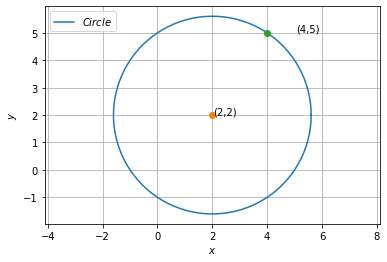
\includegraphics[width=\columnwidth]{solutions/july/2/2/Figures/Figure.png}
    \caption{Plot of the required circle}
    \label{quadforms/july/2/2/Figure}
\end{figure}

\item Find the locus of all the unit vectors in the xy-plane.
%
\item Find the points on the curve $\vec{x}^T\vec{x}-2\myvec{1 & 0}\vec{x} -3 =0$  at which the tangents are parallel to the x-axis.
%
\item  Find the area of the region in the first quadrant enclosed by x-axis, line $\myvec{1 & -\sqrt{3}}\vec{x} =0$ and the circle $\vec{x}^T\vec{x}=4$.
%
\item Find the area lying in the first quadrant and bounded by the circle $\vec{x}^T\vec{x}=4$ and the lines $x = 0$ and $x = 2$.
%
\item Find the area of the circle $4\vec{x}^T\vec{x}=9$.
\item  Find the area bounded by curves $\norm{\vec{x}-\myvec{1\\0}} = 1$ and $\norm{\vec{x}}=1$
\item Find the smaller area enclosed by the circle $\vec{x}^T\vec{x}=4$ and the line $\myvec{1 & 1}\vec{x} = 2$.
%\item The sum of the perimeter of a circle and square is $k$, where $k$ is some constant. Prove that the sum of their areas is least when the side of square is double the radius of the circle.
%\item A window is in the form of a rectangle surmounted by a semicircular opening. The total perimeter of the window is 10 m. Find the dimensions of the window to admit maximum light through the whole opening.
%
\item If 
$
\brak{x-a}^2+\brak{y-b}^2 = c^2,
$
for some $c > 0$, prove that 
\begin{align}
\frac{\brak{1+y_2}^\frac{3}{2}}{y_2}
\end{align}
%
is a constant independent of $a$ and $b$.
%
\item Form the differential equation of the family of circles touching the y-axis at origin.
\item Form the differential equation of the family of circles having centre on y-axis and radius 3 units.
\item Form the differntial equation of the fmaily of circles touching the x-axis at the origin.
%
\item Form the differential equation of the family of circles in the second quadrant and touching the coordinate axes.
\item Factorise $y^2 – 5y + 6$.
\item Find the zeroes of the quadratic polynomial $x^2+7x+10$ and verify the relationship between the zeroes and the coefficients.


\item Find a quadratic polynomial, the sum and product of whose zeroes are – 3 and 2, respectively.
%
\item Find the roots of the equation $5x^2  – 6x – 2 = 0 $.
\item Find the roots of $4x^2 + 3x + 5 = 0 $.
\item Find the roots of the following quadratic equations, if they exist.
\begin{enumerate}
    \item
    \begin{align}
    \begin{split}
    3x^2-5x+2&=0 \label{quad/2/23/1.0.1}
    \end{split}
    \end{align}
    \item
    \begin{align}
    \begin{split}
    x^2+4x+5&=0 \label{quad/2/23/1.0.2}
    \end{split}
    \end{align}
    \item 	$2x^2-2\sqrt{2}x+1 = 0$
\end{enumerate}
%
\solution
\begin{enumerate}

Let the given Matrix be
\begin{equation}
\vec{A} = \myvec{3&5\\1&1}
\end{equation}
Transposing the above matrix gives,
\begin{equation}
\vec{A}^{\top} = \myvec{3&1\\5&1}
\end{equation}
Now, for Symmetric and Skew Symmetric Matrix,
\begin{align}
    \vec{B} &= \frac{\vec{A} + \vec{A}^{\top}}{2} = \myvec{3&3\\3&1} \\
    &= \vec{B}^{\top}
\end{align}
Also,
\begin{align}
    \vec{C} &= \frac{\vec{A} - \vec{A}^{\top}}{2} = \myvec{0&2\\-2&0} \\
    &= -\vec{C}^{\top}
\end{align}

Hence, $\vec{B}$ is a Symmetric Matrix and $\vec{C}$ is a Skew Symmetric Matrix and $\vec{B} + \vec{C} = \vec{A}$.
\begin{align}
    \therefore \myvec{3&5\\1&1} = \myvec{3&3\\3&1} + \myvec{0&2\\-2&0}  
\end{align}




\end{enumerate}

\item Solve $x^2+ 2 = 0 $.
\item Solve $x^2+ x+1 = 0 $.
\item Solve $\sqrt{5}x^2+ x+\sqrt{5} = 0 $.
%
\item Find the coordinates of the focus, axis, the equation of the directrix and latus rectum of the parabola $y^2 = 8x$.
%

\item Find the equation of the parabola which is symmetric about the y-axis, and passes through the point \myvec{2\\–3}.
\item Find the coordinates of the foci, the vertices, the length of major axis, the minor axis, the eccentricity and the latus rectum of the ellipse 
%
\begin{align}
\vec{x}^T\myvec{\frac{1}{25} & 0 \\ 0 & \frac{1}{9}}\vec{x} = 1
\end{align}
%
\item Find the coordinates of the foci, the vertices, the lengths of major and minor axes and the eccentricity of the ellipse 
%
\begin{align}
\vec{x}^T\myvec{9 & 0 \\ 0 & 4}\vec{x} = 36
\end{align}
%
\item Find the equation of the ellipse whose vertices are $\myvec{\pm 13\\ 0}$ and foci are $\myvec{\pm 5\\ 0}$.
%
\item Find the equation of the ellipse, whose length of the major axis is 20 and foci are $\myvec{0\\ \pm 5}$
%

\item Find the equation of the hyperbola with  vertices $\myvec{0 \\ \pm \frac{\sqrt{11}}{2}}$, foci $\myvec{ 0\\ \pm 3}$
\item Find the equation of the hyperbola with   foci $\myvec{ 0\\ \pm 12}$ and length of latus rectum 36.
%

\item Find the roots of the following equations:
\begin{enumerate}
\item  $x + \frac{1}{x} = 3, x \ne =0 $
\item  $ \frac{1}{x} + \frac{1}{x-2}=3, x\ne =0, 2 $
\end{enumerate}
%
\solution
\begin{enumerate}
\item 
Let the given Matrix be
\begin{equation}
\vec{A} = \myvec{3&5\\1&1}
\end{equation}
Transposing the above matrix gives,
\begin{equation}
\vec{A}^{\top} = \myvec{3&1\\5&1}
\end{equation}
Now, for Symmetric and Skew Symmetric Matrix,
\begin{align}
    \vec{B} &= \frac{\vec{A} + \vec{A}^{\top}}{2} = \myvec{3&3\\3&1} \\
    &= \vec{B}^{\top}
\end{align}
Also,
\begin{align}
    \vec{C} &= \frac{\vec{A} - \vec{A}^{\top}}{2} = \myvec{0&2\\-2&0} \\
    &= -\vec{C}^{\top}
\end{align}

Hence, $\vec{B}$ is a Symmetric Matrix and $\vec{C}$ is a Skew Symmetric Matrix and $\vec{B} + \vec{C} = \vec{A}$.
\begin{align}
    \therefore \myvec{3&5\\1&1} = \myvec{3&3\\3&1} + \myvec{0&2\\-2&0}  
\end{align}




\end{enumerate}


\item Find points on the curve 
$
\vec{x}^T\myvec{\frac{1}{4} & 0 \\ 0 & \frac{1}{25}}\vec{x} = 1
$
at which the tangents are 
\begin{enumerate}
\item parallel to x-axis
\item parallel to y-axis
\end{enumerate}
 
\item Find the area enclosed by the ellipse
$
\vec{x}^T\myvec{\frac{1}{a^2} & 0 \\ 0 & \frac{1}{b^2}}\vec{x} = 1
$
%
\item Find the area of the region bounded by the curve $y = x^2$
and the line $y = 4$.
%
\item Find the area bounded by the ellipse
$
\vec{x}^T\myvec{\frac{1}{a^2} & 0 \\ 0 & \frac{1}{b^2}}\vec{x} = 1
$
and $x = ae$, where, $b^2 = a^2 (1 – e^2 )$ and $e < 1$.
%
\item Prove that the curves $y^2 = 4x$ and $x^2 = 4y$ divide the area of the square bounded by $x = 0, x = 4, y =4$ and $y = 0$ into three equal parts.
%
\item Find the area of the region
\begin{align}
\cbrak{\brak{x,y} = 0\le y\le x^2+1, 0\le y \le x+1, 0 \le x \le 2}
\end{align}

%\item Find the shortest distance of the point $\myvec{0\\c}$ from the parabola $y = x^2$, where $\frac{1}{2} \le c \le 5$.
%
%\item An apache helicopter of enemy is flying along the curve given by $y = x^2+7$.  A soldier, placed at \myvec{3\\7}, wants to shoot down the helicopter when it is nearest to him.  Find  the nearest distance.
%
\item Examine whether the function $f$ given by $f(x) = x^2$ is continuous at $x = 0$.
%
\item Discuss the continuity of the function $f$ defined by 
%
\begin{align}
f(x)  = 
\begin{cases}
x & x \ge 0
\\
x^2 & x < 0
\end{cases}
\end{align}
%
\item Verify Rolle's theorem for the function $y = x^2+2, a = -2$ and $b = 2$.
\item Verify Mean Value Theorem for the function $f(x) = x^2$ in the interval $\sbrak{2,-4}$.
%\end{align}
\item Find the derivative of $f(x) = x^2$.
\item Find the derivative of $ x^2 - 2$ at $x = 10$.
\item Find the derivative of $ \brak{x-1} \brak{x-2}$.
%
%
\item Find 
\begin{align}
\int_{0}^{2} \brak{x^2+1}\,dx
\end{align}
%
as a limit of a sum.
\item Evaluate the following integral:
%
\begin{align}
\int_{2}^{3}x^2 \,dx
\end{align}
%
\item Form the differntial equation representing the family of ellipses having foci on x-axis and cenre at the origin.
%
\item Form the differntial equation representing the family of parabolas having vertex at origin and axis along positive direction of x-axis.
\item Form a differntial equation representing the following family of curves
%
\begin{align}
y^2 = a\brak{b^2-x^2}
\end{align}
%
\item  A cricket ball is thrown at a speed of 28 $m s^{-1}$
in a direction 30$\degree$ above
the horizontal. Calculate 
\begin{enumerate}
\item  the maximum height, 
\item  the time taken by the ball to return to the same level, and 
\item  the distance from the thrower to the point where the ball returns to the same level.
\end{enumerate}
\item Find the roots of the equation  $2x^2– 5x + 3 = 0$ .
\item Find the value of  the following polynomial at the indicated value of variables 
\begin{align}
p(x) = 5x^2– 3x + 7 \text{  at } x = 1.
\end{align}
%\end{enumerate}
 
\input{./conics/conics_exer.tex} 
\end{enumerate}
\section{Appendices}
\subsection{Roots of a quadratic equation}
\input{app/1/ChallengeProblem3.tex} 
\subsection{Axes of a conic}
\input{app/2/ChallengeProblem5.tex} 


%
%
\end{document}


